%%%%%%%%%%%%%%%%%%%%%%%%%%%%%%%%%%%%%%%%%%%%%%%%%%%%%%%%%%%%%%%%%%%%%%%%%%%
%                                                                         %
%			TEMPLATE LATEX PER TESI                                       %
%			______________                                                %
%                                                                         %
%           Ultima revisione: 13 aprile 2023                              %
%           Revisori: G.Presti; L.A.Ludovico; F. Avanzini; M. Tiraboschi, %
%                     Marco Aceti                                         %
%                                                                         %
%%%%%%%%%%%%%%%%%%%%%%%%%%%%%%%%%%%%%%%%%%%%%%%%%%%%%%%%%%%%%%%%%%%%%%%%%%%

\documentclass[12pt,italian]{report}
\usepackage{template}
\usepackage[colorinlistoftodos]{todonotes}


% CORSO DI LAUREA:
\def\myCDL{Corso di Laurea in Informatica}

% TITOLO TESI:
\def\myTitle{Trasporto ferroviario e Open Data}

% AUTORE:
\def\myName{\textbf{Marco Aceti}}
\def\myMat{Matr.\ 963032}

% RELATORE E CORRELATORE:
\def\myRefereeA{Prof.\ Andrea Trentini}

% ANNO ACCADEMICO
\def\myYY{2022-2023}

% Il seguente comando introduce un elenco delle figure dopo l'indice (facoltativo)
%\figurespagetrue

% Il seguente comando introduce un elenco delle tabelle dopo l'indice (facoltativo)
%\tablespagetrue

%
%			PREAMBOLO
%

% Package di formato
\usepackage[a4paper]{geometry}		% Formato del foglio
\usepackage[italian]{babel}			% Supporto per l'italiano
\usepackage[utf8]{inputenc}			% Supporto per UTF-8
%\usepackage[a-1b]{pdfx}			% File conforme allo standard PDF-A (obbligatorio per la consegna)

% Package per la grafica
\usepackage{graphicx}				% Funzioni avanzate per le immagini
\usepackage{hologo}					% Bibtex logo with \hologo{BibTeX}
\usepackage{enumitem}

% Citazioni e bibliografia
\usepackage[style=italian]{csquotes}
\usepackage[backend=biber,style=numeric,sorting=none]{biblatex}
\addbibresource{bibliografia.bib}
\usepackage[toc]{appendix}

% Package tipografici
\usepackage{lmodern,textcomp}		% Latin Modern font
\usepackage{amssymb,amsmath,amsthm} % Simboli matematici
\usepackage{listings}				% Scrittura di codice
\usepackage{minted}                 % Scrittura di codice

% Sistema note a pié di pagina nelle tabelle
\usepackage{footnote}
\makesavenoteenv{tabular}
\makesavenoteenv{table}

% Package ipertesto
\usepackage{url}					% Visualizza e rendere interattii gli URL
\usepackage{hyperref}				% Rende interattivi i collegamenti interni

% Path immagini
\graphicspath{ {./images/} }

\begin{document}

% Creazione automatica del frontespizio
\frontespizio \beforepreface

% DEDICA
\hfill
\begin{minipage}{15cm}
	\hfill
	\begin{minipage}[t]{11cm}
		\raggedleft \large { \sl

			Nei confronti di Trenord \\
			sono state usate espressioni violente come \\
			``disastro, incubo, degrado, punizione''. \\
			\bigskip
			Abbiamo sempre rispettato le opinioni di tutti,\\
			ma dinanzi a tanta accanita disinformazione crediamo
            doveroso rivolgerci direttamente a voi, clienti e
            viaggiatori, per darvi i dati reali di quanto accaduto ed
            offrirvi le corrette spiegazioni.

			\bigskip }
	\end{minipage} \\
	\raggedleft \large
	% \textbf{-- Paolo Garavaglia} \\
	% \textrm{Direttore Comunicazioni e Relazioni Esterne, Trenord} \\

	\textbf{Trenord, Lettera ai clienti} \\
	Milano, 2 febbraio 2022
\end{minipage}
	
% \prefacesection{Ringraziamenti} Questa sezione, facoltativa,
% contiene i ringraziamenti.
	
\afterpreface
	
\listoftodos
	
\chapter{Introduzione}

Ad oggi in Italia non esistono Open Data generalizzati sulla
\textit{reale} performance del \textbf{trasporto pubblico
    ferroviario}; l'accesso a tali metriche è ostacolato da
\textbf{barriere tecnologiche e legali}, spesso ingiustificate.  Le
poche e frammentate statistiche pubblicamente disponibili su eventi
come \textit{ritardi} o \textit{cancellazioni} sono spesso
arbitrariamente aggregate, impedendo l'uso di strumenti di analisi
avanzati.

\textit{Come può un Cittadino, quindi, valutare l'operato delle
    imprese ferroviarie e degli enti committenti senza l'accesso ai
    \textbf{dati reali} sul servizio?}

Il lavoro di tesi si articola sull’idea di \textbf{preservare i dati
    istantanei} della circolazione ferroviaria dalla piattaforma
ViaggiaTreno per produrre Open Data storici, \textit{machine-readable}
e di qualità.  Inoltre, verranno proposte a fini dimostrativi alcune
analisi dei dati raccolti.

\section{Il trasporto ferroviario in Italia}

Sul territorio nazionale sono previsti due soggetti distinti che
operano sulla ferrovia:
\begin{itemize}
	\item le \textbf{imprese ferroviarie}, ovvero \textcquote[art.\ 2,
    comma 1, lettera a)]{Dlgs112}{qualsiasi impresa pubblica o privata
        titolare di una licenza, la cui attività principale consiste
        nella prestazione di servizi per il trasporto sia di merci sia
        di persone per ferrovia e che garantisce obbligatoriamente la
        trazione};
	\item i \textbf{gestori dell'infrastruttura}, ovvero
    \textcquote[art.\ 2, comma 1, lettera b)]{Dlgs112}{qualsiasi
        organismo o impresa responsabili dell'esercizio, della
        manutenzione e del rinnovo dell'infrastruttura ferroviaria di
        una rete nonché della partecipazione al suo sviluppo come
        stabilito dallo Stato nell'ambito della sua politica generale
        sullo sviluppo e sul finanziamento dell'infrastruttura}.
\end{itemize}

\subsection{Le Società sul territorio}

Attualmente sono certificate 18 \textbf{imprese ferroviarie} per il
servizio passeggeri \cite{ElencoIF}, tra cui Trenitalia S.p.A.,
Trenord S.r.l.\ e Trenitalia Tper S.C.a.R.L.  Il principale
\textbf{gestore dell'infrastruttura} è Rete Ferroviaria Italiana
S.p.A.\ (RFI, 16829 km \cite{RfiKm}), seguito da Ferrovie Emilia
Romagna (343 km \cite{FerKm}) e Ferrovienord (330 km
\cite{FerNordKm}).  Il gruppo \textbf{Ferrovie dello Stato Italiane
    S.p.A.} è una partecipata del Ministero dell'Economia e delle
Finanze \cite{MefGruppoFS} e controlla totalmente alcune delle Società
già citate, come Trenitalia S.p.A.\ e Rete Ferroviaria Italiana
S.p.A.\ \cite{ControllateFS}.

\subsubsection{Lombardia}

Trenord S.r.l.\ è una \textit{joint venture}\footnote{Contratto di
    accordo tra due o più imprese al fine di raggiungere un obiettivo
    comune} di Trenitalia (al 50\%) e il gruppo FNM S.p.A.\
(FerrovieNord Milano, al 50\%) \cite{TrenordChiSiamo}.  Quest'ultimo è
posseduto da Regione Lombardia (al 57,57\%) e da Trenitalia stessa (al
14,74\%); il restante 27,69\% è quotato in Borsa
\cite{BorsaItalianaFNM}.  La bizzarra composizione societaria cela una
totale partecipazione di Trenitalia S.p.A.\ del $\sim 57\%$, di
Regione Lombardia del $\sim 28$\% e del restante $\sim 15\%$ da parte
di azionisti privati.  L'infrastruttura è gestita sia da RFI\ (1740 km
\cite{RfiKm}) che da Ferrovienord (controllata da FNM, 330 km
\cite{FerNordKm}).

\subsubsection{Emilia-Romagna}

La Trenitalia Tper S.C.a.R.L.\ è una società consortile partecipata da
Trenitalia S.p.A.\ (al 70\%) e TPER S.p.a.\ (Trasporto Passeggeri
Emilia-Romagna, al 30\%) \cite{NascitaTper}; quest'ultima è a sua
volta ripartita tra diversi soggetti pubblici dell'Emilia Romagna
\cite{SociTper}.  Similmente alla Lombardia, l'infrastruttura è
gestita sia da RFI (1319 km \cite{RfiKm}) che da FER S.r.l.\
(controllata dalla Regione \cite{FerChiSiamo}, 343 km \cite{FerKm}).

\subsection{Il servizio pubblico e il mercato}

La fornitura del servizio di trasporto ferroviario passeggeri è
costituita da \textbf{offerte a mercato} (treni ad alta velocità) e
\textbf{contratti di servizio pubblico}, stipulati dalle imprese
ferroviarie con lo Stato (per le tratte a media e lunga percorrenza) o
con le Regioni (per le connessioni regionali e interregionali)
\cite[vedi][paragrafo \textit{``Gli obblighi di servizio pubblico e i
    contratti di servizio''}]{CameraTrasportoFerroviario}.

Il servizio pubblico può essere oggetto di \textbf{compensazioni
    economiche} da parte dell'Ente, ma queste devono essere
commisurate in base a dei \textbf{parametri ben definiti} \cite[art.\
4, comma 1]{Reg1370}.  Fino al 25 dicembre 2023 permane la possibilità
delle autorità di affidare direttamente i contratti di servizio
pubblico, senza gara \cite[art.\ 8, comma 2, lettera iii)]{Reg1370}.

Il quadro normativo evidenzia la \textbf{funzione pubblica} del
servizio di trasporto ferroviario regionale e interregionale, esente
dalle normali logiche di libero mercato ma
\textcquote{CameraTrasportoFerroviario}{\textit{funzionale ad
        assicurare \textbf{il diritto costituzionale alla mobilità}}}.
La forte responsabilità politica degli enti committenti nel definire
concessioni, contratti di servizio e compensazioni ha un grande
impatto sulla qualità del trasporto ferroviario, sia in termini di
programmazione che di \textit{performance}.

\subsection{Performance regime}

Ogni anno, RFI pubblica il c.d.\ PIR (Prospetto Informativo della
Rete) per comunicare alle imprese ferroviarie le modalità e le tariffe
di assegnazione della capacità dell'infrastruttura per l'erogazione
dei servizi \cite{RfiPir}.  %Nel PIR viene inoltre
definito un complesso sistema di \textbf{penali}, calcolate in base a
metriche ben precise (e spesso richiamate da numerosi contratti di
servizio) qui di seguito esposte. \\ Nel PIR viene inoltre descritta
la c.d.\ \textbf{\textit{performance regime}}, un meccanismo di premi
e penali adottata \textcquote[art.\ 21]{Dlgs112}{\textit{al fine di
        ridurre al minimo le disfunzioni conseguenti ad eventuali
        perturbazioni arrecate alla circolazione dei treni}}.
	
\subsubsection{Metodo di calcolo delle penali}

La metrica alla base del calcolo della performance di regime è il
c.d.\ \textbf{scostamento}, ovvero la differenza in minuti tra
l'orario di passaggio reale del treno in una \textit{stazione
    rilevante} e l'orario programmato \cite[app.\ 5.C,
\textit{``Definizioni''}]{RfiPir}.  Ad ogni scostamento maggiore di 2
minuti o dovuto ad anormalità deve essere attribuita una \textbf{causa
    di ritardo}, riconducibile al gestore dell'infrastruttura,
all'impresa ferroviaria, ad altra impresa ferroviaria o forza
maggiore.  Al fine di calcolo delle penali vengono utilizzati i
seguenti \textbf{coefficienti} \cite[app.\ 5.C, \textit{``Metodi di
    calcolo''}]{RfiPir}:

\begin{itemize}
	\item $P_\text{u}$: penale unitaria pari a 1,00€ al minuto;
	\item $P_\text{sop}$: penale unitaria per ogni treno soppresso
    pari a $120 P_\text{u}$;
	\item $C_\text{t}$: tipologia di linea \cite[app.\ 5C, tabella
    1]{RfiPir};
	\item $C_\text{cat}$: categoria del treno \cite[app.\ 5C, tabella
    4]{RfiPir};
	\item $C_\text{rit}$: ritardo complessivo della corsa \cite[app.\
    5C, tabelle 2a, 2b, 2c]{RfiPir};
	\item $C_\text{sop}$: stato di soppressione \cite[app.\ 5C,
    tabella 6]{RfiPir};
	\item $C_\text{ser}$: tipologia di servizio \cite[app.\ 5C,
    tabella 3]{RfiPir};
\end{itemize}

Dall'\textbf{insieme degli scostamenti} $S$ sono definite le seguenti
metriche:

\begin{itemize}
	\item $M_\text{GI} : S \rightarrow \mathbb N^+$ minuti di ritardo
    attribuiti al gestore dell'infrastruttura;
	\item $M_\text{FI} : S \rightarrow \mathbb N^+$: minuti di ritardo
    attribuiti all'impresa ferroviaria;
	\item $M_{a, b} : S \rightarrow \mathbb N^+$: minuti di ritardo
    attribuiti all'impresa ferroviaria $a$ provocati ai treni
    dell'impresa $b$.
\end{itemize}

Per le \textbf{soppressioni} sono definite ulteriori metriche:
\begin{itemize}
	\item $S_\text{GI}$: numero di treni con provvedimento di
    soppressione, anche parziale, per responsabilità del gestore
    dell'infrastruttura;
	\item $P_\text{GI}$: rapporto tra treni-km soppressi per
    responsabilità del gestore dell'infrastruttura e treni-km
    programmati;
	\item $S_{a, b}$: numero di treni dell'impresa ferroviaria $b$ con
    provvedimento di soppressione, anche parziale, per responsabilità
    dell'impresa ferroviaria $a$;
	\item $P_{a, b}$: rapporto tra treni-km dell'impresa ferroviaria
    $b$ soppressi per responsabilità dell'impresa $a$ e treni-km
    programmati.
\end{itemize}

Le \textbf{penali} sono pertanto corrisposte tramite tre flussi
indipendenti:

\begin{itemize}[noitemsep]
	\item \textbf{da gestore dell'infrastruttura a impresa
        ferroviaria}
	\begin{align*} P_\text{F1} &= P_\text{u} \cdot \sum_{s \in S}
        \left ( M_\text{GI}(s) \cdot C_\text{t} \cdot C_\text{cat}
            \cdot C_\text{rit} \right) + P_\text{sop} \cdot
        S_\text{GI} \cdot P_\text{GI} \cdot C_\text{sop};
        \intertext{\item \textbf{da impresa ferroviaria al gestore
                dell'infrastruttura}} P_\text{F2} &= P_\text{u} \cdot
        \sum_{s \in S} \left ( M_\text{FI}(s) \cdot C_\text{t} \cdot
            C_\text{ser} \cdot C_\text{car} \cdot C_\text{rit} \right
        ); \intertext{\item \textbf{da impresa ferroviaria ad altra
                impresa ferroviaria}} P_\text{F3} &= P_\text{u} \cdot
        \sum_{s \in S} \left ( M_{a,b}(s) \cdot C_\text{t} \cdot
            C_\text{cat} \cdot C_\text{rit} \right ) + P_\text{sop}
        \cdot S_{a,b} \cdot P_{a,b} \cdot C_\text{sop}.
	\end{align*}
\end{itemize}

Intuitivamente, le cancellazioni di treni per colpa delle imprese
ferroviarie proprietarie non causano penali nei confronti del gestore
dell'infrastruttura, ma invertendo le responsabilità sì.

\subsubsection{Flusso economico}

È bene notare come \textcquote{RfiPir}{\textit{il flusso economico
        annuo tra GI\footnote{Gestore dell'Infrastruttura} e ogni
        singola IF\footnote{Impresa Ferroviaria} non potrà superare il
        valore del 5\% del totale del pedaggio consuntivato nel corso
        dell’anno}}. Nel caso dovesse registrarsi un importo a favore
del GI, l'80\% di tale somma verrà \textbf{ridistribuita} alle altre
IF proporzionalmente in base a un punteggio
$$
t \cdot (C_\text{base} + C_\text{correttivo}),
$$
dove $t$ è il volume di treni-km commerciali sviluppati in puntualità
dall'IF, $C_\text{base}$ si basa sull'\textit{incremento} dell'indice
di puntualità rispetto all'anno precedente \cite[app.\ 5C, tabella
5a]{RfiPir} e $C_\text{correttivo}$ sull'\textbf{indice di puntualità}
dell'anno in esame \cite[app.\ 5C, tabella 5b]{RfiPir}.  Quest'ultimo
è definito come il rapporto tra il numero di treni giunti a destino
entro una certa soglia (5' per i treni passeggeri, 30' per i merci) e
il numero totale dei treni circolanti della stessa IF.  Nell'indice
sono comunque considerati \textit{puntuali} i treni giunti a destino
oltre soglia a causa del GI, di altra IF o eventi di forza maggiore.

In sintesi, il sistema di ridistribuzione delle penali premia le
imprese ferroviarie più virtuose ($C_\text{correttivo}$)
incentivandole a migliorare ($C_\text{base}$) al fine di aumentare la
\textbf{performance regime} complessiva.

\section{Infrastruttura tecnologica}

La circolazione ferroviaria è regolata dal gestore
dell'infrastruttura.  All'interno delle stazioni e in linea esistono
dei sistemi (come i \textbf{circuiti di binario}) in grado di
stabilire se un tratto di binario è occupato o libero.  All'inizio di
una corsa, un operatore \textit{``battezza''} un tratto occupato
inserendo il numero di treno corrispondente.  Man mano che il treno
occupa e libera altri tratti di binario adiacenti, il \textbf{sistema
    informatico} lo segue.  In questo modo, il gestore
dell'infrastruttura conosce sempre la posizione aggiornata di tutti i
treni sulle proprie linee.

Lo stato dei treni viene quindi trasmesso alle imprese ferroviarie che
lo elaborano e lo comunicano ai viaggiatori attraverso siti web e
applicazioni.

\subsection{Portale Viaggiatreno}
\label{viaggiatreno}

\begin{figure}[h] \centering
    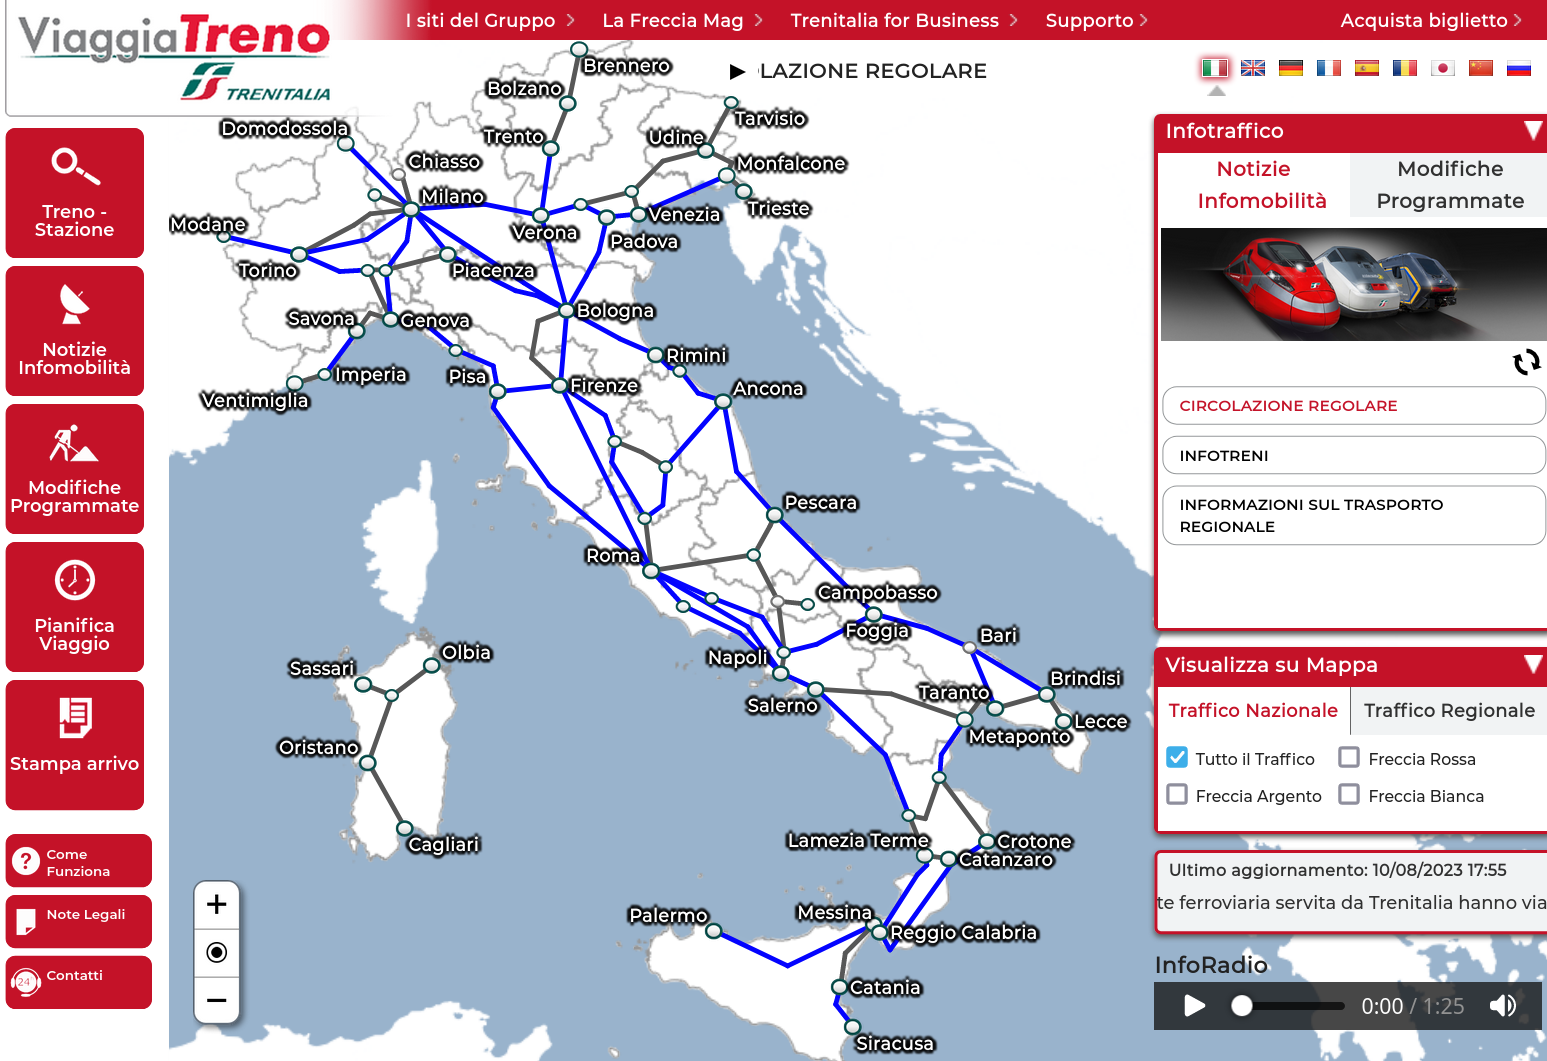
\includegraphics[width=1\textwidth]{images/viaggiatreno.png}
	\caption{Homepage di Viaggiatreno}
\end{figure}

Il portale Viaggiatreno\footnote{https://viaggiatreno.it} è stato
sviluppato da Trenitalia ed è attivo almeno dal
2006\footnote{Informazione ricavata dal \texttt{whois} del dominio}.
Il sito web permette numerose operazioni, come:
\begin{itemize}
	\item \textbf{cercare un treno} per numero o itinerario e
    visualizzare il ritardo, le fermate, luogo e orario di ultimo
    rilevamento;
	\item \textbf{cercare una stazione} per nome e visualizzare
    partenze e arrivi;
	\item \textbf{leggere o ascoltare le informazioni sulla mobilità}
    (Infomobilità).
\end{itemize}

La caratteristica più interessante ai fini del progetto è la
possibilità di operare anche tramite delle semplici \textbf{API HTTP},
senza autenticazione o apparenti limiti tecnologici.  Utilizzando lo
strumento \textit{``Ispeziona elemento''} di un qualsiasi browser è
possibile tracciare le richieste invocate dal frontend in JavaScript a
seguito delle azioni dell'utente e farsi un'idea dei metodi API
disponibili.

Con Viaggiatreno è possibile trovare le corse di Trenitalia
(regionali, alta velocità, Intercity e Intercity Notte), Trenord, TPER
e OBB (Ferrovie Austriache).  Curiosamente, non è possibile cercare i
treni di Italo-NTV, concorrente commerciale del gruppo Ferrovie dello
Stato.

\subsection{Sito web di Trenord}

\begin{figure}[h]
	\centering
    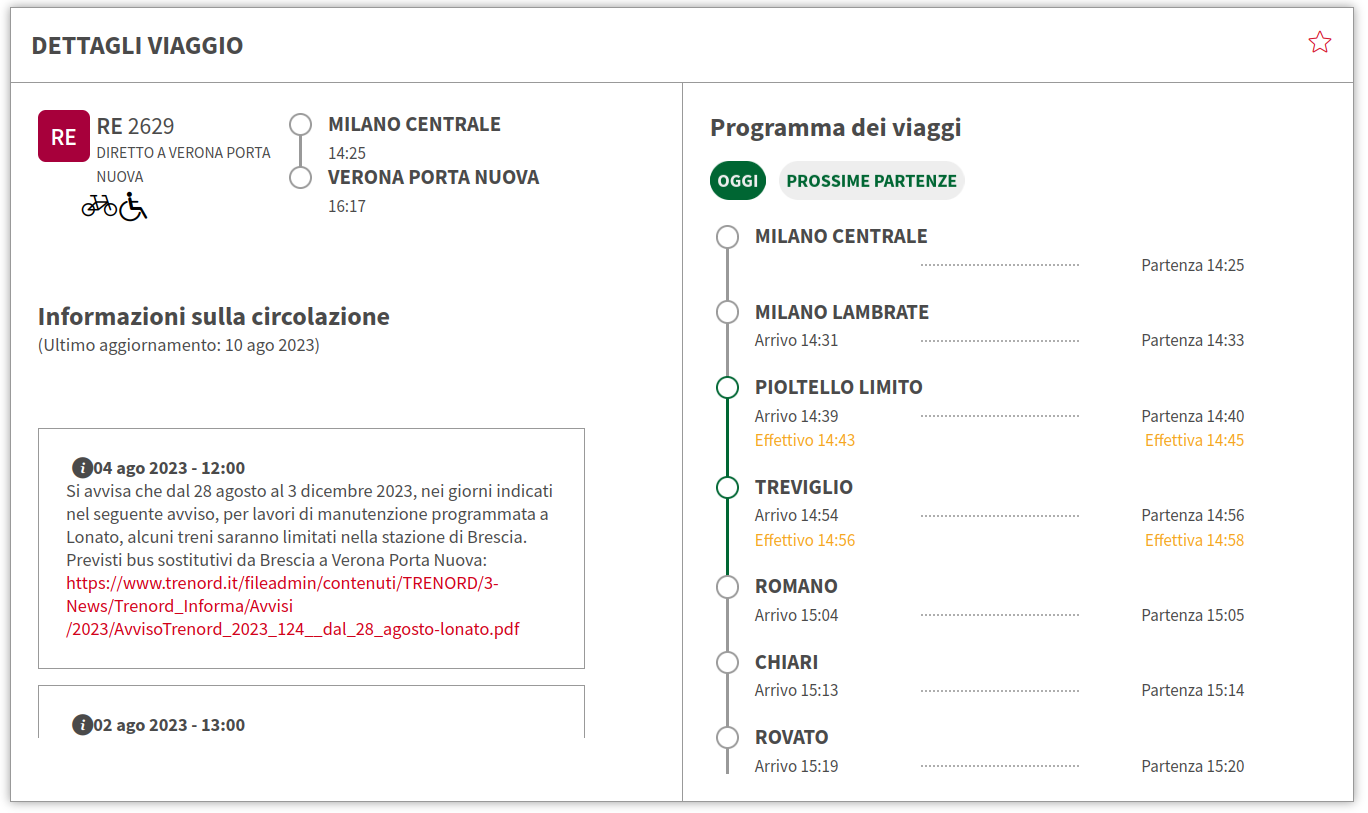
\includegraphics[width=1\textwidth]{images/trenord_api.png}
	\caption{Dettagli di una corsa sul portale web di Trenord}
\end{figure}

Trenord mette a disposizione ai viaggiatori un'applicazione mobile e
un portale web per consultare lo stato dei treni in circolazione e gli
arrivi e le partenze di una stazione.

Similmente a Viaggiatreno, con lo strumento \textit{``Ispeziona
    elemento''} si possono facilmente individuare delle \textbf{API
    HTTP} sotto la URL \texttt{https://admin.trenord.it}.  Nonostante
l'assenza di una documentazione ufficiale, l'interazione con le API
Trenord è più intuitiva e prevedibile rispetto a quelle di
Viaggiatreno.  Le risposte sono sempre in JSON e le richieste seguono
i principi REST di HTTP GET.

Dai portali di Trenord non si trovano corse non operate dall'impresa
stessa, come i regionali di Trenitalia o l'alta velocità.  Nonostante
ciò, le API Trenord si sono rilevate utili per verificare e correggere
alcune incongruenze riscontrate in quelle di Viaggiatreno. \\

In Appendice \ref{documentazione} sono documentati alcuni metodi
rilevanti delle due API.

\printbibliography

\addcontentsline{toc}{chapter}{Bibliografia}

\appendix

\chapter{Documentazione}
\label{documentazione}

\section{Terminologia}
\label{terminologia}

Prima di analizzare le API occorre fissare alcuni termini e concetti
fondamentali, sorprendentemente spesso controintuitivi.

Una \textbf{stazione} è un \textit{luogo di sosta temporanea} per i
convogli ferroviari.  Ha un \textit{nome} e uno o più \textit{codici}
corrispondenti, utilizzati per identificarla.  I nomi delle stazioni
non necessariamente rispettano i nomi delle località in cui sono
situate e una città può naturalmente includere più stazioni.  In
alcuni casi l'API ritorna ``stazioni'' non più attive o inesistenti,
come posti di movimento o depositi ferroviari.

Con il termine \textbf{treno} si intende la \textit{corsa di un
    convoglio ferroviario}.  I treni che non fanno servizio
viaggiatori sono oltre gli obiettivi del progetto.  Ogni treno ha una
\textit{numero}, una \textit{origine}, una \textit{destinazione}, una
collezione ordinata di \textit{fermate intermedie} e altre proprietà
che verranno approfondite nei prossimi capitoli.  Il numero di treno
non è un \textbf{identificatore univoco} e non può essere utilizzato
come tale, in quanto può essere riassegnato a treni di altre imprese
ferroviarie.  La stessa \textit{corsa} può variare tra giornate
diverse, sia per motivi programmati (per esempio, fermate
straordinarie nel weekend) che non (treni parzialmente soppressi).  Un
treno è univocamente identificato dalla tripla
$(\texttt{Data}, \, \texttt{Origine}, \, \texttt{Numero})$.

Una \textbf{fermata} è una stazione in cui un treno, oltre che a
transitare, \textit{sosta}.  L'\textit{origine} e la
\textit{destinazione} sono considerarsi fermate particolari: un treno
sosta quindi in almeno due fermate, la prima e l'ultima.  Ad ogni
fermata è associato un \textit{orario programmato} ed
\textit{effettivo} di arrivo e partenza la cui differenza è il
relativo ritardo.  La prima fermata non può avere un orario di arrivo
e viceversa.  Le fermate possono essere ordinarie, straordinarie o
soppresse.  Un treno avente alcune fermate sorppresse è detto
\textit{parzialmente soppresso}, uno con tutte \textit{soppresso}.

\section{API di Viaggiatreno}

Le API di Viaggiatreno (vedi la Sezione \ref{viaggiatreno}) non
dispongono di una documentazione ufficiale e non sono conformi alla
architettura REST o ad altri standard \textit{de facto} \cite{Giunta}.
Numerosi tentativi sono stati fatti dalla comunità open source
italiana per documentarle: in particolare ringrazio Stefano (sabas)
\cite{Sabas}, Luca Grandi \cite{Grandi} e Fabrizio Tarizzo
\cite{Tarizzo} per il loro fondamentale contributo.  I metodi sono
generalmente accessibili al percorso
\texttt{/infomobilita/\-resteasy/\-viaggiatreno/\-$M$/\-$P_1$/\-$P_2$/\-$\dots$/\-$P_n$}
dove $M$ è il nome del metodo e $P_1, P_2, \dots, P_n$ i suoi
parametri. A seconda della richiesta l'API può rispondere in JSON o in
altri formati \textit{plain text}.


\subsection{\texttt{/cercaStazione/<nome>}}

Il metodo ritorna \textit{tutte le stazioni} cui nome inizia con il
nome indicato.  Per ogni stazione viene ritornato il suo codice, un
nome ``lungo'' e uno ``breve'' e il nome della città in cui si trova.

\subsubsection{Esempio}

$\Rsh$ \texttt{/cercaStazione/MILANO}
\begin{minted}{js}
[
  {
    "nomeLungo": "MILANO CENTRALE", // nome lungo
    "nomeBreve": "Milano Centrale", // nome breve (può essere nullo)
    "label": "Milano",              // città (può essere nullo)
    "id": "S01700"                  // codice stazione
  },
  // ...
]
\end{minted}

\subsubsection{Avvertenze}

Il metodo non restituisce tutte le stazioni.  Ad esempio, la stazione
di Arcene (BG) non viene mai ritornata, neanche cercandola dal sito
web.  L'unico modo per reperire il suo ID è consultare le fermate di
un treno in corsa.

\subsection{\texttt{/regione/<codiceStazione>}}

Il metodo ritorna il codice della regione di appartenza della stazione
richiesta.  Il contenuto della risposta, in testo semplice, può essere
utilizzato nel metodo successivo.

\begin{table}[h] \centering
    \begin{tabular}{r|l}
      Codice & Nome \\
      \hline
      1 & Lombardia \\
      2 & Liguria \\
      3 & Piemonte \\
      4 & Valle D'Aosta \\
      5 & Lazio \\
      6 & Umbria \\
      7 & Molise \\
      8 & Emilia Romagna \\
      9 & Trentino-Alto Adige \\
      10 & Friuli Venezia Giulia \\
      11 & Marche \\
    \end{tabular}
    \begin{tabular}{r|l}
      Codice & Nome \\
      \hline
      12 & Veneto \\
      13 & Toscana \\
      14 & Sicilia \\
      15 & Basilicata \\
      16 & Puglia \\
      17 & Calabria \\
      18 & Campania \\
      19 & Abruzzo \\
      20 & Sardegna \\
      21 & Trentino-Alto Adige \\
      22 & Trentino-Alto Adige
    \end{tabular}
    \caption{Codici API delle regioni italiane}
    \label{regioni}
\end{table}

\subsubsection{Esempio}

$\Rsh$ \texttt{/regione/S01700} \hfill (Milano Centrale)
\begin{minted}{text}
1
\end{minted}

\subsubsection{Avvertenze}

Osservando la Tabella \ref{regioni} si può notare che le stazioni
della regione Trentino-Alto Adige assumono 3 codice regione
differenti, senza nessun pattern apparente.  Non tutte le stazioni
sono riconosciute, specialmente quelle in gestione a Ferrovienord.  In
tal caso, la risposta dell'API è \texttt{0}.

\subsection{\texttt{/elencoStazioni/<codiceRegione>}}

Il metodo ritorna tutte le stazioni della regione data.  Con il codice
\texttt{0} vengono ritornate solo le stazioni principali.  La
funzionalità è presumibilmente utilizzata per popolare la mappa
presente in homepage.

La risposta è in formato JSON e per ogni elemento viene fornito un
superinsieme di informazioni rispetto a \texttt{cercaStazione}, come
la latitudine e longitudine.

\subsubsection{Esempio}

$\Rsh$ \texttt{/elencoStazioni/3} \hfill (Piemonte)
\begin{minted}{js}
[
 {
    "codReg": 3,  // Codice regione
    "tipoStazione": 3,
    "dettZoomStaz": [  // (può non essere presente)
      {
        "codiceStazione": "S01013",
        "zoomStartRange": 8,
        "zoomStopRange": 9,
        "pinpointVisibile": true,
        "pinpointVisible": true,
        "labelVisibile": true,
        "labelVisible": true,
        "codiceRegione": null
      },
      {
        "codiceStazione": "S01013",
        "zoomStartRange": 10,
        "zoomStopRange": 11,
        "pinpointVisibile": true,
        "pinpointVisible": true,
        "labelVisibile": true,
        "labelVisible": true,
        "codiceRegione": null
      }
    ],
    "pstaz": [],
    "mappaCitta": {
      "urlImagePinpoint": "",
      "urlImageBaloon": ""
    },
    "codiceStazione": "S01013",
    "codStazione": "S01013",
    "lat": 45.943821,  // Latitudine (può essere nullo)
    "lon": 8.47224,  // Longitudine (può essere nullo)
    "latMappaCitta": 0,
    "lonMappaCitta": 0,
    "localita": {  // Medesime proprietà di cercaStazione
      "nomeLungo": "VERBANIA-PALLANZA",
      "nomeBreve": "Verbania",
      "label": "Verbania-Pallanza",
      "id": "S01013"
    },
    "esterno": false,
    "offsetX": -4,
    "offsetY": 10,
    "nomeCitta": "Verbania"  // Vedere avvertenze
  }, ...
]
\end{minted}

\subsubsection{Avvertenze}

Il campo \texttt{nomeCitta} può essere nullo oppure ``\texttt{A}''
(stesso significato).  Sono generalmente ritornate più stazioni
rispetto a \texttt{cercaStazione}, ma comunque non tutte: le stazioni
senza informazioni sulla localizzazione, come Aiello (UD), sono
ignorate \textit{in toto}.  Alcune ``stazioni'' sono punti di appoggio
per generare la mappa e sono da ignorare: si distinguno in quanto
hanno \texttt{tipoStazione} uguale a ``\texttt{4}''.  Infine, esistono
stazioni figuranti in più regioni contemporaneamente: per esempio, la
stazione di Casalmaggiore (CR) risulta essere sia in Lombardia che in
Emilia Romagna.  Verificando con \texttt{/regione}, però, la stazione
risulta correttamente in Lombardia.

\subsection{\texttt{/<partenze|arrivi>/<orarioAttuale>}}

I metodi \texttt{partenze} e \texttt{arrivi} ritornano i treni in
partenza o in arrivo della stazione data.  Il campo
\texttt{orarioAttuale} è da indicare nel formato \texttt{\%a \%b \%d
    \%Y \%H:\%M:\%S \%Z\%z} e non può essere diverso dall'orario in
cui si invia la richiesta.

La risposta è in formato JSON e contiene molte informazioni sia sul
treno che sulla \textit{fermata} nella stazione richiesta.

\subsubsection{Esempio}

$\Rsh$ \texttt{/partenze/S01700/Wed Mar 08 2023 17:04:00 GMT+0100}
\hfill (Milano Centrale) \\

\noindent \textit{La risposta è nello stesso formato degli elementi
    dell'array \texttt{fermate} documentato con il metodo
    \texttt{andamentoTreno} (\ref{andamentoTreno}) --- è quindi stata
    omessa.}

\subsection{\texttt{/cercaNumeroTrenoTrenoAutocomplete/<numeroTreno>}}
\label{trenoAutocomplete}

Come detto precedentemente (\ref{terminologia}), un treno è
univocamente identificabile dalla combinazione del suo numero, origine
e data di partenza.  Il metodo
\texttt{cerca\-Numero\-Treno\-Treno\-Autocomplete} serve per
disambugare treni aventi lo stesso numero, ritornando il codice della
stazione di origine e il
\textit{timestamp}\footnote{\label{timestamp}Tutti i timestamp
    dell'API di Viaggiatreno sono intesi come \textit{numero di
        \textbf{millisecondi} passati dal 1° gennaio 1970}, nel fuso
    orario locale.} della mezzanotte del giorno di partenza della
corsa.

La risposta è in \texttt{text/plain} e non rispetta formati standard
(JSON, XML, CSV, \dots).

\subsubsection{Esempio}

$\Rsh$ \texttt{/cercaNumeroTrenoTrenoAutocomplete/2107}

\begin{minted}{text}
2107 - TORINO PORTA NUOVA|2107-S00219-1678230000000
2107 - MILANO NORD CADORNA|2107-N00001-1678230000000
\end{minted}

Il primo risultato è un regionale di Trenitalia da Torino P.N., il
secondo è un Malpensa Express di Trenord da Milano Nord Cadorna.

\subsection{\texttt{/andamentoTreno/<origine>/<numero>/<data>}}
\label{andamentoTreno}

Il metodo \texttt{andamentoTreno} fornisce tutte le informazioni su un
treno e le sue fermate.  L'\texttt{origine} è il codice della stazione
cui il treno ha origine, \texttt{numero} è il numero del treno e
\texttt{data} è il timestamp della mezzanotte del giorno di partenza
del treno, ritornato dal metodo precedente (\ref{trenoAutocomplete}).

Il JSON risultante contiene molti campi ridondanti o sempre nulli, con
nomi inconsistenti e a volte bizzarri.  Molti di essi non sono
documentabili, in quanto mancano evidenze del loro utilizzo.

I campi cui nome inizia con ``\texttt{comp}'' sembrano essere rivolti
alla UI di Viaggiatreno, in quanto i loro valori sono più
\textit{human-friendly}. Quelli terminanti con ``\texttt{Zero}''
marcano le informazioni originali -- pertanto obsolenn te -- prima di una
riprogrammazione (come la soppressione di alcune fermate).

\subsubsection{Esempio}

$\Rsh$ \texttt{/andamentoTreno/S01717/10124/1692136800000} \hfill (REG
10124 da Brescia)

\begin{minted}[texcomments=true]{js}
{
  "tipoTreno": "PG",
  "orientamento": null,
  "codiceCliente": 63,  // Impresa ferroviaria, vedi Tabella \ref{codice_cliente}
  "fermateSoppresse": null,
  "dataPartenza": null,
  "fermate": [  // Lista delle fermate
    // ...
    {
      "orientamento": null,
      "kcNumTreno": null,
      "stazione": "OSPITALETTO TRAVAGLIATO",  // Nome della fermata
      "id": "S01716",  // Codice della stazione della fermata
      "listaCorrispondenze": null,
      "programmata": 1692180300000,  // Vedi arrivo\_teorico
      "programmataZero": null,
      "effettiva": 1692180300000,  // Vedi arrivo\_effettivo
      "ritardo": 0,  // Vedi ritardoArrivo
      "partenzaTeoricaZero": null,
      "arrivoTeoricoZero": null,
      "partenza_teorica": 1692180360000,  // Orario di partenza programmato
      "arrivo_teorico": 1692180300000,  // Orario di arrivo programmato
      "isNextChanged": false,
      "partenzaReale": 1692180420000,  // Orario di partenza effettivo
      "arrivoReale": 1692180300000,  // Orario di arrivo effettivo
      "ritardoPartenza": 1,  // Ritardo in partenza
      "ritardoArrivo": 0,  // Ritardo in arrivo
      "progressivo": 3,  // Numero progressivo della fermata
      "binarioEffettivoArrivoCodice": "4663",
      "binarioEffettivoArrivoTipo": "0",
      "binarioEffettivoArrivoDescrizione": "2"  // Binario di arrivo
      "binarioProgrammatoArrivoCodice": null,
      "binarioProgrammatoArrivoDescrizione": null,
      "binarioEffettivoPartenzaCodice": "4694",
      "binarioEffettivoPartenzaTipo": "0",
      "binarioEffettivoPartenzaDescrizione": "2",  // Binario di partenza
      "binarioProgrammatoPartenzaCodice": null,
      "binarioProgrammatoPartenzaDescrizione": null,
      "tipoFermata": "F",  // Tipologia di fermata, vedi Tabella \ref{tipo_fermata}
      "visualizzaPrevista": true,
      "nextChanged": false,
      "nextTrattaType": 0,
      "actualFermataType": 1,
      "materiale_label": null
    },
    // ...
  ],
  "anormalita": null,
  "provvedimenti": null,
  "segnalazioni": null,
  "oraUltimoRilevamento": 1692180630000,  // Orario ultimo rilevamento
  "stazioneUltimoRilevamento": "ROVATO",  // Ultimo punto di rilevamento
  "idDestinazione": "S01529",  // Codice della stazione di destinazione
  "idOrigine": "S01717",  // Codice della stazione di origine
  "cambiNumero": [],
  "hasProvvedimenti": false,
  "descOrientamento": [
    "--",
    "--",
    "--",
    "--",
    "--",
    "--",
    "--",
    "--",
    "--"
  ],
  "compOraUltimoRilevamento": "12:10",  // Orario ultimo rilevamento
  "motivoRitardoPrevalente": null,
  "descrizioneVCO": "",
  "materiale_label": null,
  "numeroTreno": 10124,  // Numero treno
  "categoria": "REG",  // Categoria del treno
  "categoriaDescrizione": null,
  "origine": "BRESCIA",  // Nome della stazione di origine
  "codOrigine": null,
  "destinazione": "BERGAMO",  // Nome della stazione di destinazione
  "codDestinazione": null,
  "origineEstera": null,
  "destinazioneEstera": null,
  "oraPartenzaEstera": null,
  "oraArrivoEstera": null,
  "tratta": 0,
  "regione": 0,
  "origineZero": "BRESCIA",  // Origine originale, se tr. parzialmente soppresso
  "destinazioneZero": "BERGAMO",  // Destinazione originale, se "
  "orarioPartenzaZero": 1692179820000,  // Orario partenza originale, se "
  "orarioArrivoZero": 1692183240000,  // Orario arrivo originale, se "
  "circolante": true,  // true se il treno è in circolazione
  "binarioEffettivoArrivoCodice": null,
  "binarioEffettivoArrivoDescrizione": null,
  "binarioEffettivoArrivoTipo": null,
  "binarioProgrammatoArrivoCodice": null,
  "binarioProgrammatoArrivoDescrizione": null,
  "binarioEffettivoPartenzaCodice": null,
  "binarioEffettivoPartenzaDescrizione": null,
  "binarioEffettivoPartenzaTipo": null,
  "binarioProgrammatoPartenzaCodice": null,
  "binarioProgrammatoPartenzaDescrizione": null,
  "subTitle": "",
  "esisteCorsaZero": "0",
  "inStazione": false,  // true se il treno è in sosta presso una fermata
  "haCambiNumero": false,
  "nonPartito": false,
  "provvedimento": 0,  // $\neq 0$ se cancellato
  "riprogrammazione": null,
  "orarioPartenza": 1692179820000,  // Orario di partenza programmato
  "orarioArrivo": 1692183240000,  // Orario di arrivo programmato
  "stazionePartenza": null,
  "stazioneArrivo": null,
  "statoTreno": null,
  "corrispondenze": null,
  "servizi": [],
  "ritardo": -1,  // Ritardo reale, aggiornato ai punti di rilevamento
  "tipoProdotto": "0",
  "compOrarioPartenzaZeroEffettivo": "11:56",
  "compOrarioArrivoZeroEffettivo": "12:54",
  "compOrarioPartenzaZero": "11:57",
  "compOrarioArrivoZero": "12:54",
  "compOrarioArrivo": "12:54",
  "compOrarioPartenza": "11:57",
  "compNumeroTreno": "REG 10124",
  "compOrientamento": [
    "--",
    "--",
    "--",
    "--",
    "--",
    "--",
    "--",
    "--",
    "--"
  ],
  "compTipologiaTreno": "regionale",
  "compClassRitardoTxt": "",
  "compClassRitardoLine": "regolare_line",
  "compImgRitardo2": "",
  "compImgRitardo": "/vt_static/img/legenda/icone_legenda/regolare.png",
  "compRitardo": [
    "anticipo 1 min.",
    "advance 1 min.",
    "Verfr&#252hung 1 Min.",
    "avance de 1 min.",
    "adelanto de 1 min.",
    "avans 1 min.",
    "",
    "",
    ""
  ],
  "compRitardoAndamento": [
    "con un anticipo di 1 min.",
    "1 minutes early",
    "mit einem Vorsprung von 1 Min.",
    "en avance de 1 min.",
    "est&aacute; adelantado 1 min.",
    "cu un avans de 1 min.",
    "",
    "",
    "con un anticipo di 1 min."
  ],
  "compInStazionePartenza": [
    "",
    "",
    "",
    "",
    "",
    "",
    "",
    "",
    ""
  ],
  "compInStazioneArrivo": [
    "",
    "",
    "",
    "",
    "",
    "",
    "",
    "",
    ""
  ],
  "compOrarioEffettivoArrivo": "/vt_static/img/legenda/icone_legenda/regolare.png12:53",
  "compDurata": "0:57",
  "compImgCambiNumerazione": "&nbsp;&nbsp;",
  "dataPartenzaTreno": 1692136800000
}
\end{minted}

\begin{table}[h]
    \centering
    \begin{tabular}{r|l}
      Codice & Impresa ferroviaria \\
      \hline
      \texttt{1} & Trenitalia (alta velocità) \\
      \texttt{2} & Trenitalia (regionale) \\
      \texttt{4} & Trenitalia (intercity) \\
      \texttt{18} & Tper \\
      \texttt{63} & Trenord \\
      \texttt{64} & Österreichische Bundesbahnen\footnote{Ferrovie
                    federali austriache}
    \end{tabular}
    \caption{Codici delle imprese ferroviarie}
    \label{codice_cliente}
\end{table}

\begin{table}[h]
    \centering
    \begin{tabular}{r|l}
      Lettera & Tipo di fermata \\
      \hline
      \texttt{P} & Origine \\
      \texttt{F} & Fermata intermedia \\
      \texttt{A} & Destinazione \\
      \textit{(altro)} & Soppressa
    \end{tabular}
    \caption{Lettere corrispondenti alle tipologie di fermate}
    \label{tipo_fermata}
\end{table}

\subsubsection{Avvertenze}

Talvolta, nonostante il treno esista e sia già stato ritornato da
altri metodi (come \texttt{partenze}), \texttt{andamentoTreno}
risponde con HTTP 204\footnote{No Content}.  In questo caso, i
dettagli della corsa non sono disponibili.  Questo fenomeno accade
spesso con treni cancellati o riprogrammati.  \todo{Marco:
    Ricollegarsi ai ``caveats'' riscontrati nell'implementazione}

\subsection{Altri metodi}

Di seguito sono brevemente descritti altri metodi non utilizzati nel
progetto ma che potrebbero essere interessanti per estensioni future.

\begin{itemize}
    \item
    \texttt{/soluzioniViaggioNew/\-<codiceStazionePartenza>/\-<codiceStazioneArrivo>/\-<orario>}:
    trova soluzioni di viaggio tra la stazione di partenza e la
    stazione di arrivo, anche con cambi.  Per ogni soluzione è
    presente una \texttt{durata} e una lista di \texttt{vehicles} su
    cui viaggiare per arrivare a destinazione.
    \item \texttt{/statistiche/<timestamp>}: mostra il numero di treni
    circolanti al momento. Il \texttt{timestamp} deve essere quello
    attuale.
    \item \texttt{/datimeteo/\-<codiceRegione>}: restituisce i dati
    meteo delle stazioni principali della regione. Se si passa
    \texttt{0} come \texttt{codiceRegione}, vengono considerate le
    principali stazioni italiane.
\end{itemize}

\section{Metodi dell'API di Trenord}
\todo{Marco: Documentare metodi API di Trenord}

\end{document}
